\section{Result}
\label{result}

 All the tests were executed on Pianosa\footnote{Pianosa web site: \url{http://pianosa.di.unipi.it/Home_pianosa/html/info.html}}, one of the cluster of the Computer Science Department in Pisa. The cluster is composed by 24 homogeneous nodes. The nodes are 800 Mz Pentium III with 1GB of main memory and they are connected through a Fast Ethernet interconnection network. The Operating system is Fedora Core 1. On that cluster, we installed the Apache Hadoop 0.20.2 framework. The configuration parameters are set to default, so, the maximum number of task per node is set to 2 and the number of replication is set to 3. 
We decided to place the Secondary NameNode and the JobTracker in cluster interface node.
The cluster interface node is not used neither as TaskTracker nor DataNode.
21 nodes are available as slaves.

The data used in the test was generated using two matrix generators written in Matlab.
One generator for the sparse matrix A and another one for the matrices W and H. 
Both generators produce matrices containing positive elements only.
The first one is a sparse matrix generator and its sparsity factor can be tuned through an input parameter. 
The second one is dense matrix generator, the mean value of the matrix values can be selected by the user. 
For our tests, we fix the $m$ and $n$ parameters (the dimension of the A matrix) respectively to \numprint{105000} and \numprint{20000}.
All matrices value are normally distributed with a mean value of 100 and a standard deviation of 1.

For all the tests, the number of reduce task is set to $ 1,8 * number\_of\_worker$, except in the phase 3 and 4 that have 1 and 0 reducer respectively.
This choice has been driven by the Hadoop User Guide that suggest to set the reduce task number to 
$ \text{mapred.tasktracker.reduce.tasks.maximum} * number\_of\_worker * C $where C is a constant choose in the range between 0.9 and 1.8 \cite{numeroReducer}. 
The Hadoop guide claims that a value in this range should be optimal.
After a brief experimentation, we set the constant C to 0.9, a value that seem to be good for every phase.
Specifying the number of mappers is instead quite complex since the command job.setNumMapTasks give the framework only a suggestion on the number of mappers to use.
The only way to ensure that the desired number of mappers is used is to split input files accordingly. 
Therefore, the External Phase classes (that convert the input data from text to sequence) allows theuser to specify how many reducer tasks must be used. 
In that way, a corresponding number of files are produced.

The first set of tests how the computation scales in relation to the the size of the data. 
We studied how the performance change with respect to the sparsity factor of the A matrix and different k values. 
In the first test, the number of non-zero elements in the sparse matrix has been changed between \numprint{5000000} and \numprint{80000000} elements while the k parameter remain fixed to 10. 
In the second test, the k value varies between 10 and 125 while the non zero element of the A matrix has been fixed to \numprint{16500000}.  Both tests have been executed with 16 slave nodes for three iterative updates. 
The mean of the completion time for one update is reported in the Figure \ref{DeltaVar}  and \ref{kVar}. 


\begin{figure}[th]
	\centerline{
		\mbox{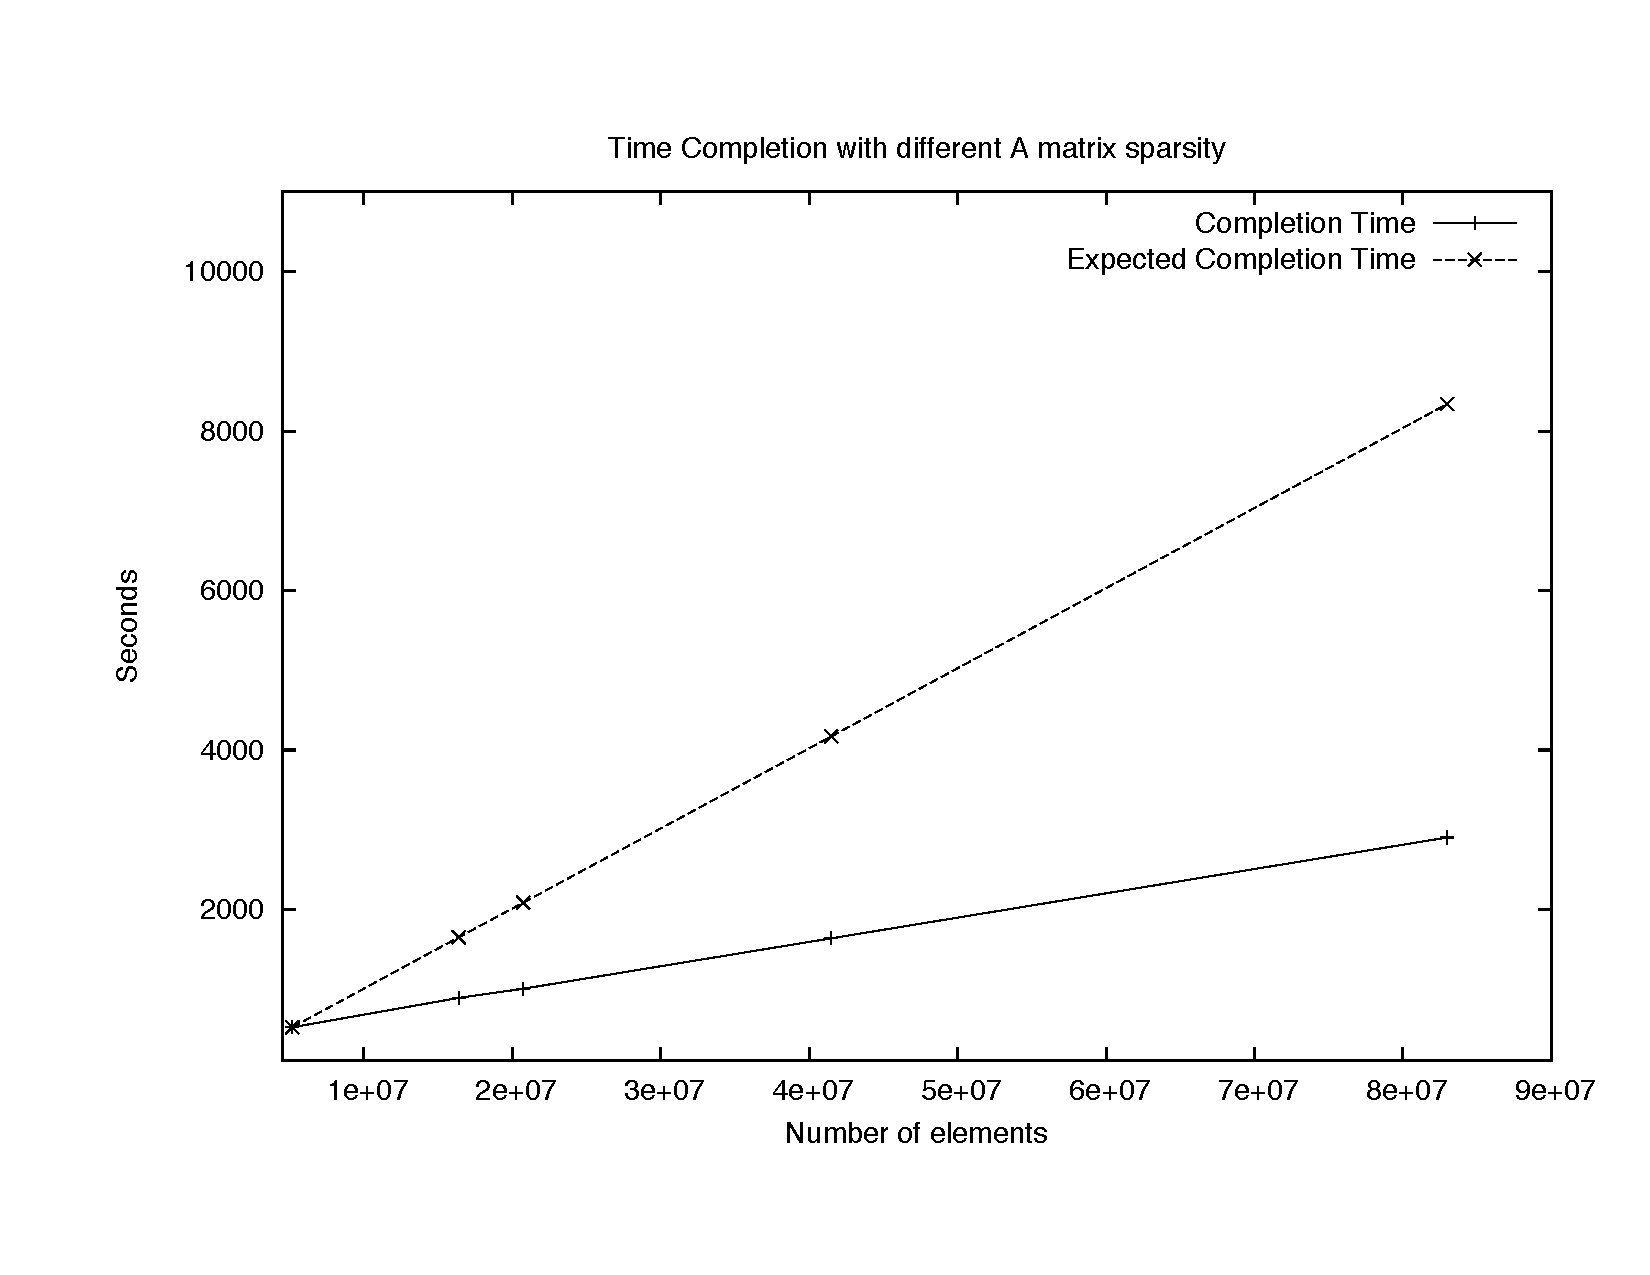
\includegraphics[scale=0.48]{HadoopTest/PsFiles/DeltaVar.pdf}}
	}
	\caption{Time Completion with different A matrix sparsity} 
        \label{DeltaVar}
\end{figure}

\begin{figure}[th]
	\centerline{
		\mbox{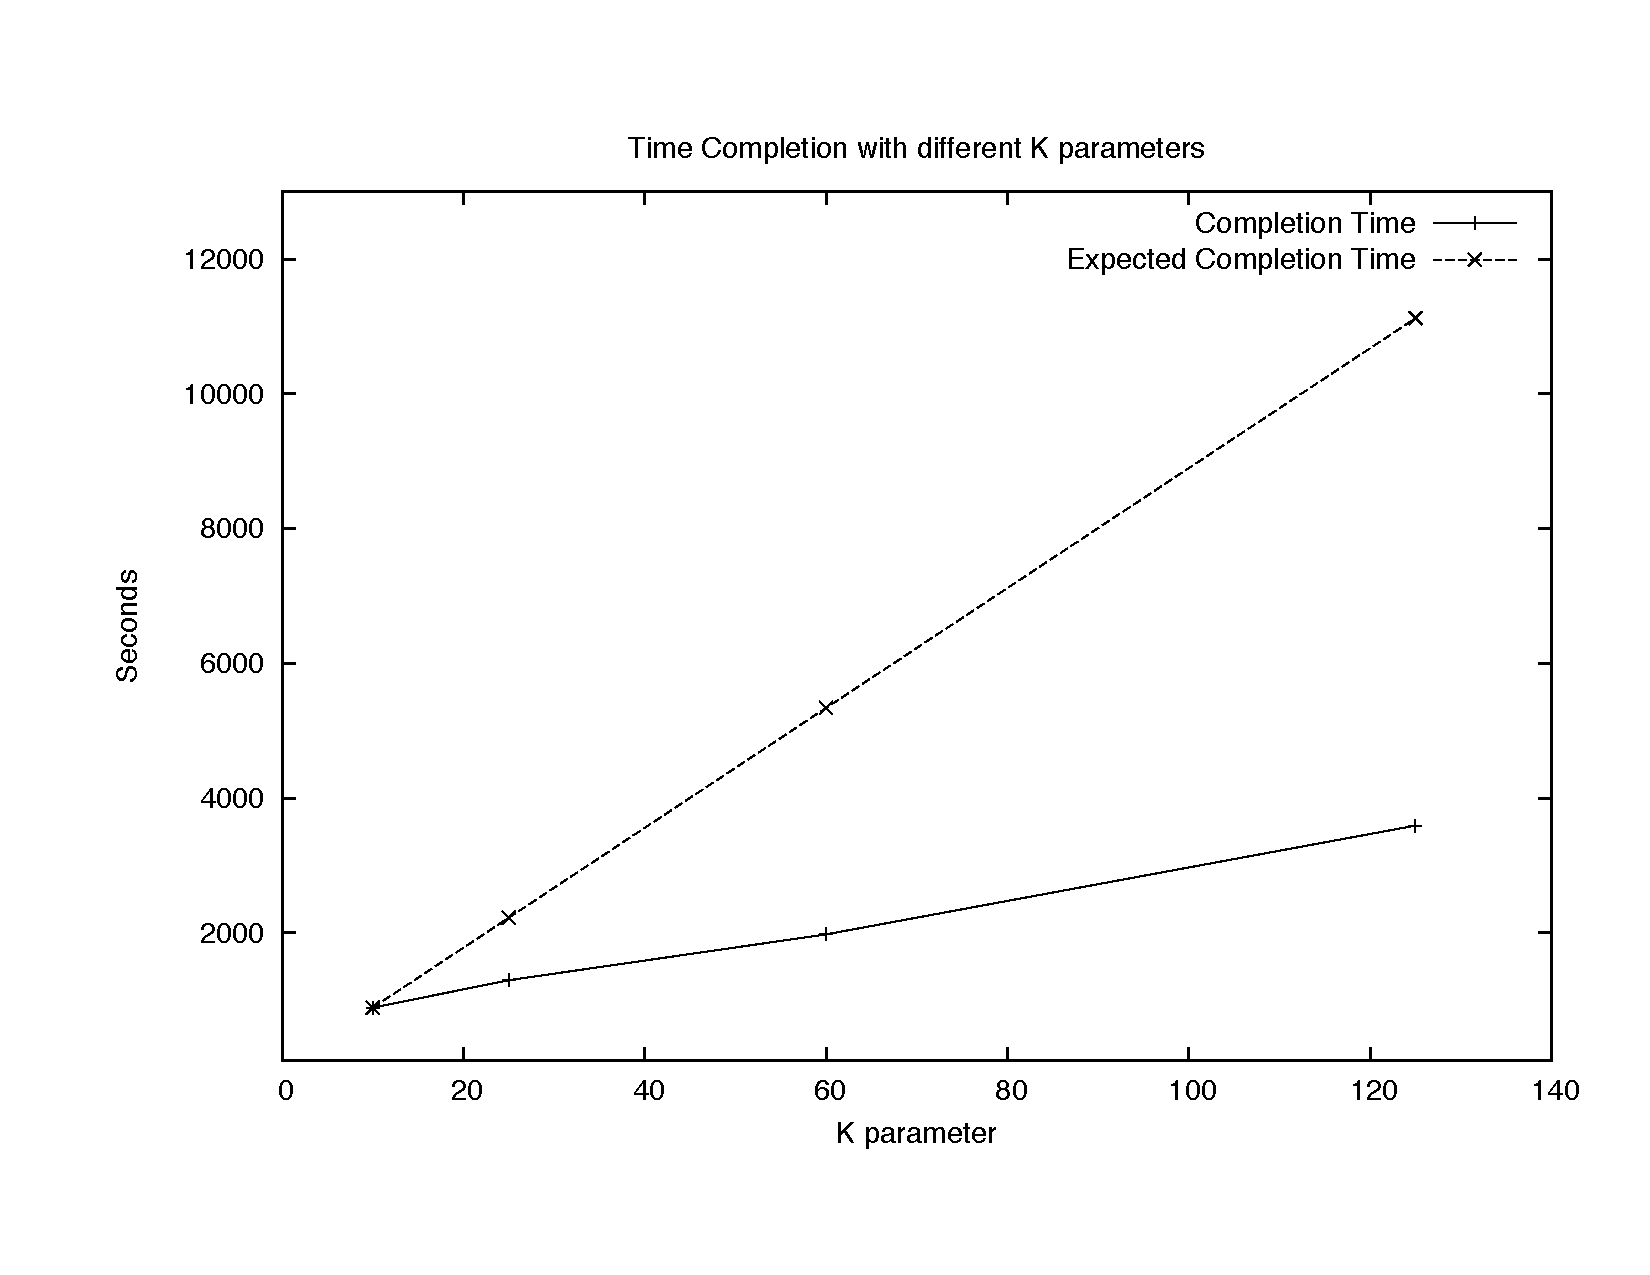
\includegraphics[scale=0.48]{HadoopTest/PsFiles/kVar.pdf}}
	}
	\caption{Time Completion with different K parameters} 
        \label{kVar}
\end{figure}


As we can see from both graphs, the behaviour of the test show a sub-linear dependencies from the size of the input data. \\

The second set of tests examines the behavior of the implementation when the parallel degree of the computation vary in the range $[1, 21]$. 
The results of the test are reported in the figure \ref{NTime}  and \ref{NScal}. 
The first graph shows completion time while the second one on the scalability.

\begin{figure}[th]
	\centerline{
		\mbox{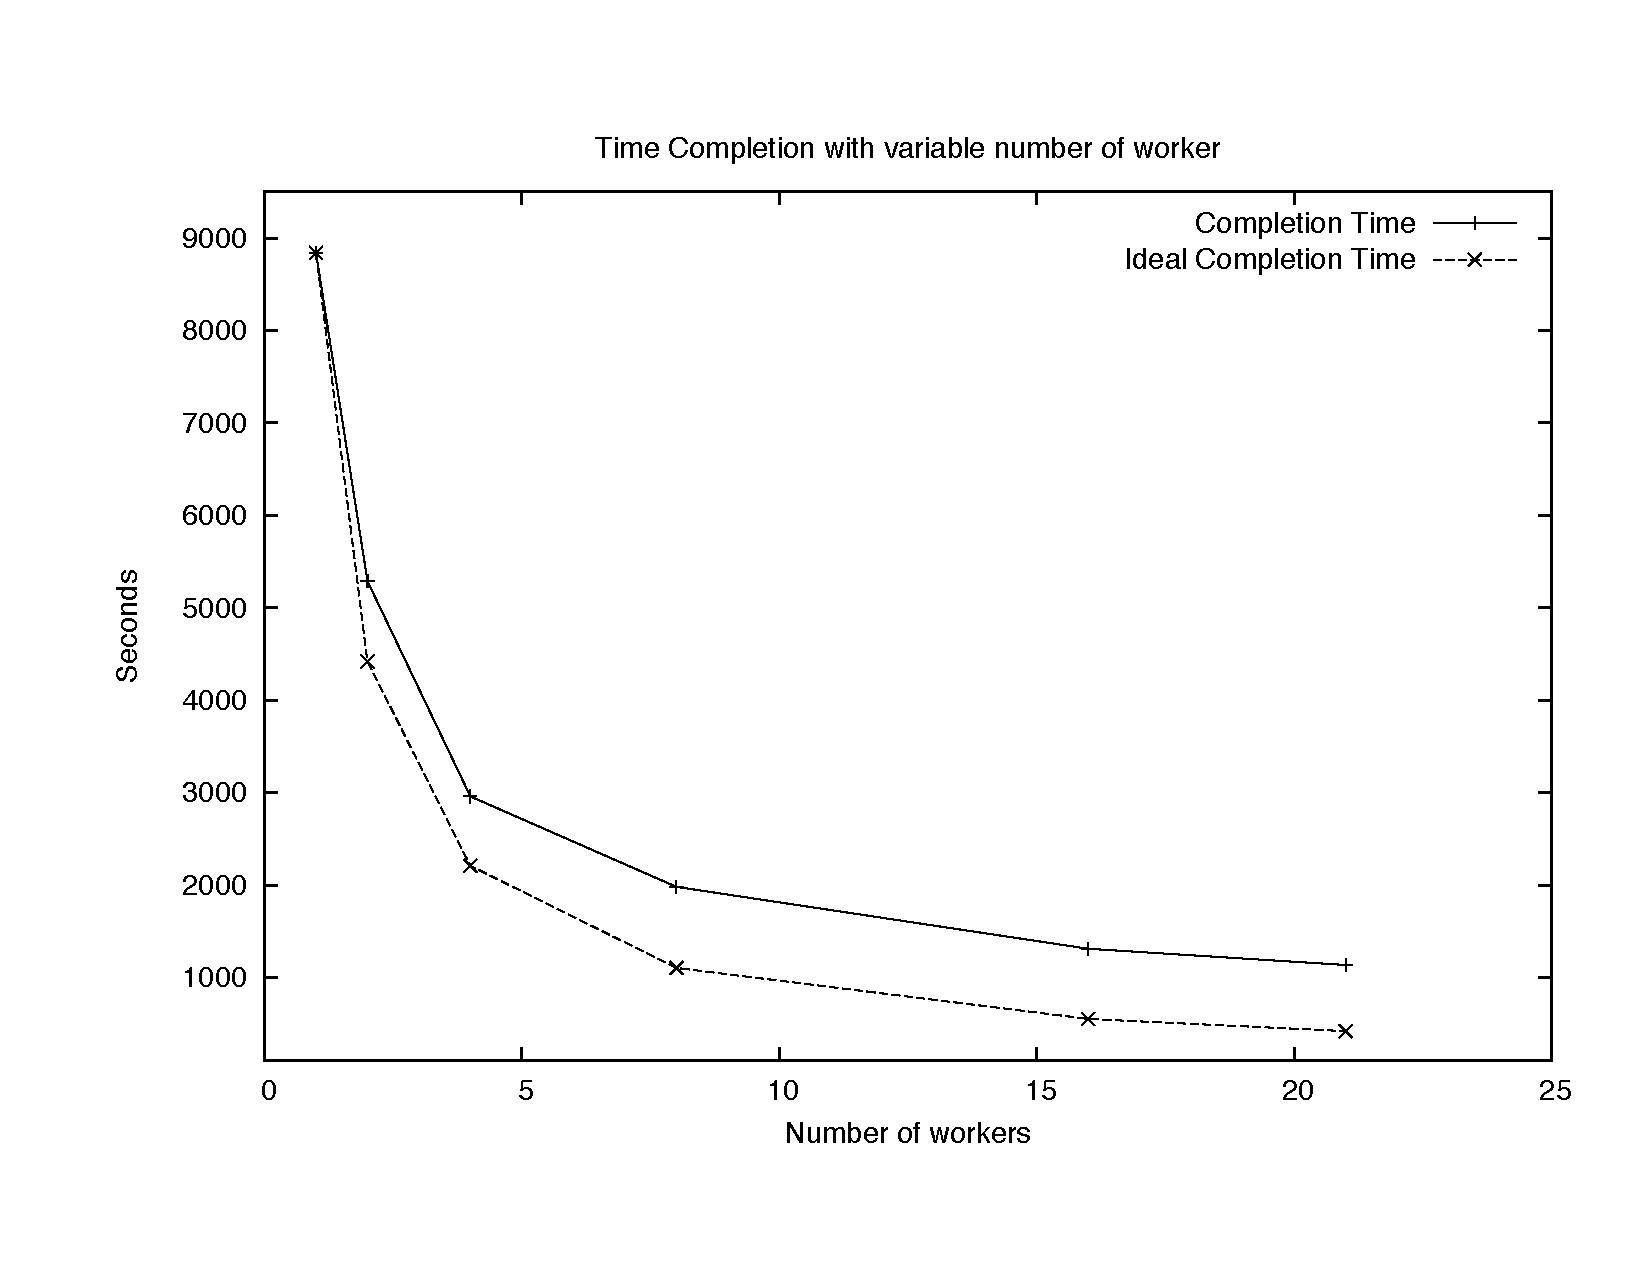
\includegraphics[scale=0.48]{HadoopTest/PsFiles/NTime.pdf}}
	}
	\caption{Time Completion with variable number of worker} 
        \label{NTime}
\end{figure}

\begin{figure}[th]
	\centerline{
		\mbox{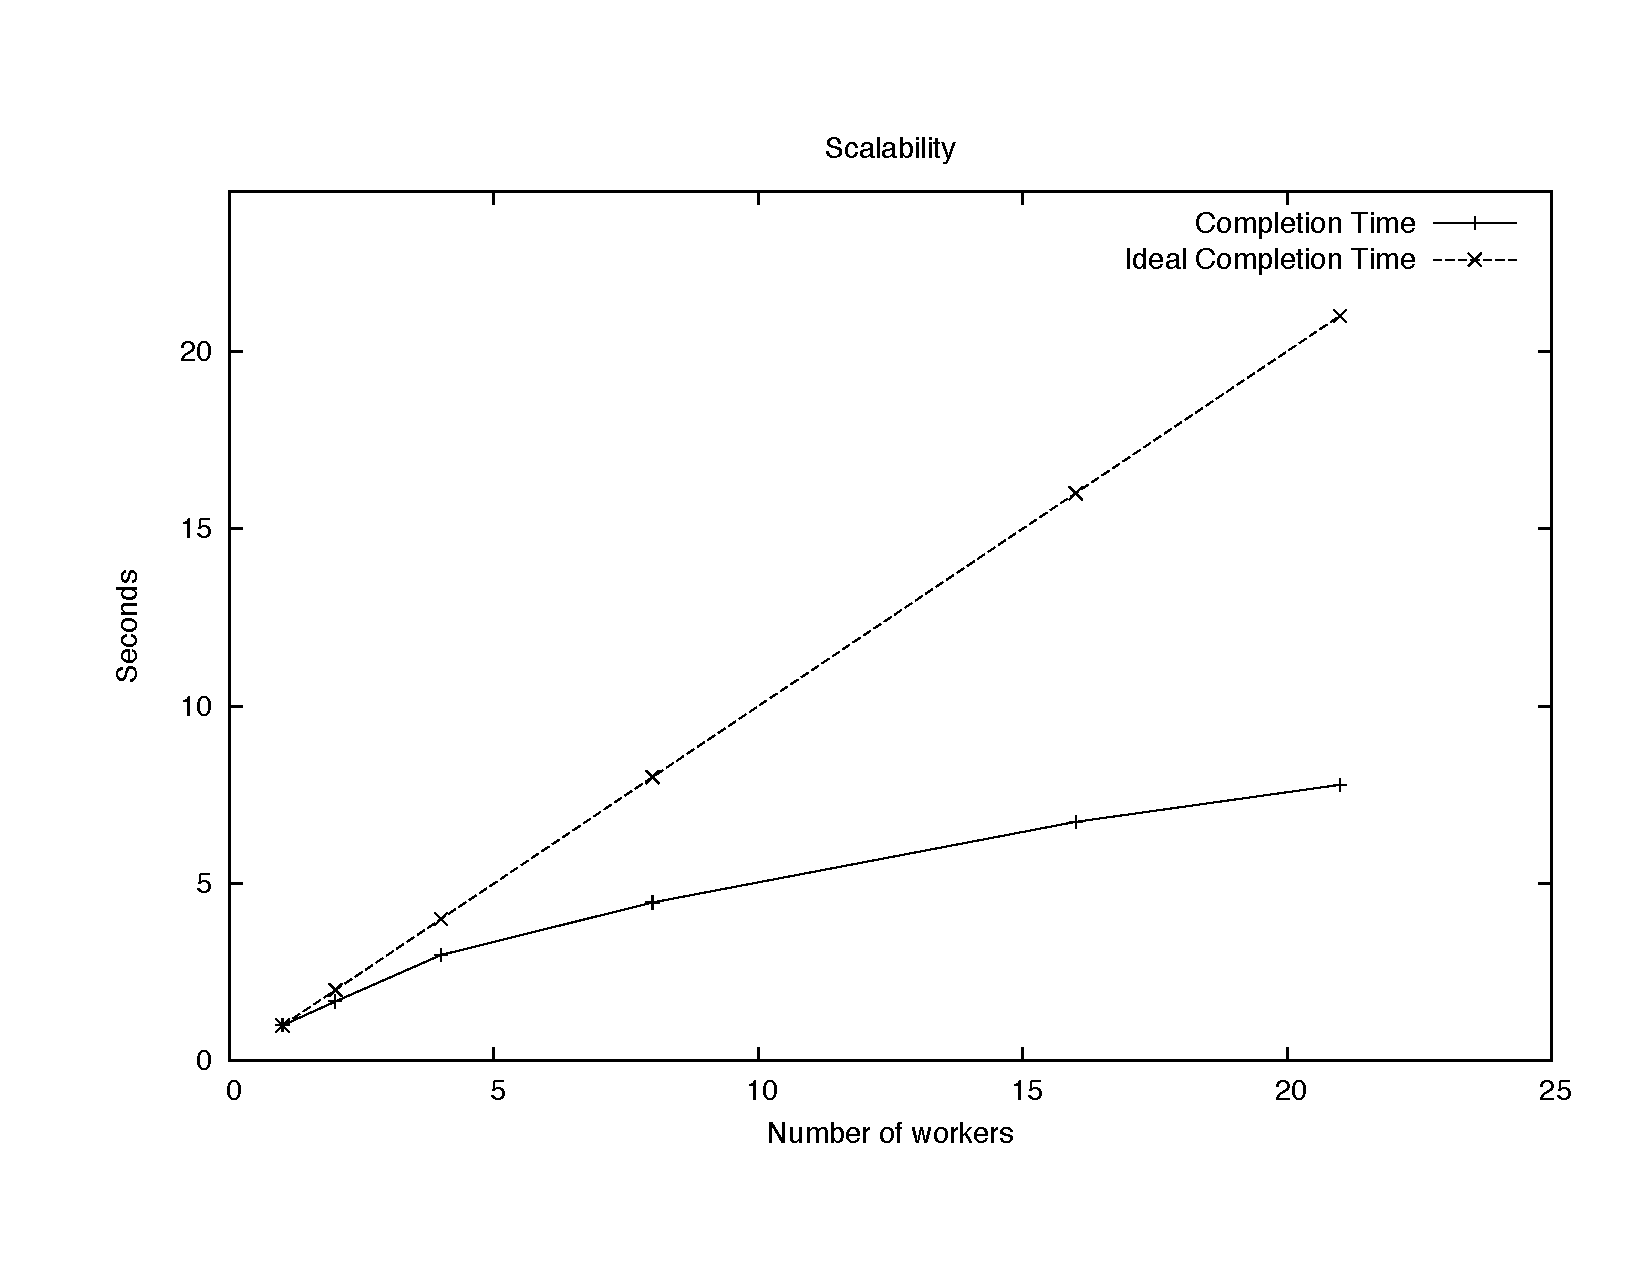
\includegraphics[scale=0.48]{HadoopTest/PsFiles/NScal.pdf}}
	}
	\caption{Scalability} 
        \label{NScal}
\end{figure}

As we can see from the figure \ref{NScal}, the implemented algorithm doesn't scale vary well. This is due mainly to two different facts: some phases in the computation doesn't scale adding more slave nodes and other phases, instead, doesn't exhibit an optimal scalability. An example of a phase that doesn't scale is the phase 5 (in which point-wise multiplication/division are done) has a minimal computational grain, both for map and reduce, and the most time spent in the computation reside in the shuffle phase. In a test we did with a parallel degree equals to 16, a shuffle task lasts in average 29 seconds, while a map and the reduce task end respectively in 8 and 3 seconds. This scenario is further compromise, taking in account that the completion time is given by the sequentialization of 5 different parallel phases. %The below table show the percentage that every phase in the computation takes varying the parallel degree.
The table reported below shows the average completion time for each phase varying the parallel degree.

\begin{center}
\begin{tabular}{ | l || c | c | c | c |  c | c | }
  \hline      
  Phase & 1 & 2 & 4 & 8 &16 & 21 \\
  \hline      
  Phase 1 & 2242 	& 1492 & 797 	& 469 	& 320 	& 304\\
  Phase 2 & 1678 	& 885 	& 478	& 217 	& 191 	& 148\\
  Phase 3 & 92 		& 66 	& 48 	& 36 	& 33 	& 30\\ 
  Phase 4 & 23 		& 19 	& 21 	& 20 	& 20 	& 20\\
  Phase 5 & 66 		& 50 	& 55 	& 55 	& 54 	& 55\\
  \hline  
\end{tabular} 
\end{center}




%\begin{center}
%\begin{tabular}{ | l || c | c | c | c |  c | c | }
%  \hline      
%  Phase & 1 & 2 & 4 & 8 &16 & 21 \\
%  \hline      
%  Phase 1 & 0,512 & 0,557 & 0,542 & 0,476 & 0,494 & 0,510\\
%  Phase 2 & 0,446 & 0,390 & 0,374 & 0,356 & 0,341 & 0,300\\
%  Phase 3 & 0,015 & 0,019 & 0,026 & 0,043 & 0,047 & 0,051\\ 
%  Phase 4 & 0,006 & 0,009 & 0,015 & 0,028 & 0,030 & 0,036\\
%  Phase 5 & 0,016 & 0,023 & 0,041 & 0,095 & 0,086 & 0,101\\
%  \hline  
%\end{tabular}
%\end{center}

Furthermore, we make additional test to verify that the assumption done during the project were verified. The first one regards the coding of the data in sequential file during the ``internal phases''. The data shown in the below table show the completion time in the case the data are represented in the sequential or textual way. We can observe that coding the data provide a lot of benefits in the completion time, especially for the phase 1 and 2.

\begin{center}
\begin{tabular}{ | l || c | c | }
  \hline      
  & Text & Sequence \\
  \hline      
  Phase 1 & 475 & 264 \\
  Phase 2 & 333 & 105 \\
  Phase 3 & 66 & 42 \\ 
  Phase 4 & 18 & 15 \\
  Phase 5 & 36 & 35 \\
  \hline  
\end{tabular}
\end{center}

The second additional test regards the combiner improvement in the completion time. The test are done taking in account the following parameters: A contains 16000000 elements, k is set to 25 and the parallel degree is 8. The below table show the result obtained by the test.

\begin{center}
\label{comb_table}
\begin{tabular}{ | l || c | c | }
  \hline      
  & \multicolumn{2}{|c|}{Record Number} \\
  & with Combiner & without Combiner \\
  \hline      
  H Phase 2 & 1896186 & 16406079 \\
  W Phase 2 & 678553 & 16406079 \\ 
  H Phase 3 & 14 & 105000 \\ 
  W Phase 3 & 14 & 20000 \\ 
 \hline  
  \hline      
  & \multicolumn{2}{|c|}{Completion Time} \\
  & with Combiner & without Combiner \\
  \hline      
  H Phase 2 & 217 & 426 \\
  W Phase 2 & 284 & 414 \\ 
  H Phase 3 & 36 & 136 \\ 
  W Phase 3 & 31 & 57 \\ 
 \hline  
\end{tabular}

\end{center}














